\documentclass[10pt]{article}
% Shared style for the RAM/SSD project documents
\usepackage[T1]{fontenc}
\usepackage[utf8]{inputenc}
%\usepackage{lmodern}
\usepackage[scaled=0.95]{helvet}
\usepackage{microtype}
\usepackage[a4paper,margin=2.2cm]{geometry}
\usepackage{xcolor}
\usepackage{graphicx}
\usepackage{booktabs}
\usepackage{tabularx}
\usepackage{array}
\usepackage[shortlabels]{enumitem}
\usepackage{titlesec}
\usepackage{fancyhdr}
\usepackage[most]{tcolorbox}
\usepackage{caption}
\usepackage[section]{placeins}
\usepackage[hidelinks]{hyperref}

\definecolor{accent}{HTML}{2A78D6}
\definecolor{ink}{HTML}{0B0B0B}
\definecolor{muted}{HTML}{52514E}
\definecolor{wash}{HTML}{F0EFEC}
\definecolor{rule}{HTML}{C3C2B7}

\hypersetup{colorlinks=true,linkcolor=accent,urlcolor=accent,citecolor=accent}
\renewcommand{\familydefault}{\sfdefault}
\setlength{\parindent}{0pt}
\setlength{\parskip}{0.55em}
\setlist{itemsep=0.2em,topsep=0.3em}

\titleformat{\section}{\color{accent}\Large\bfseries}{\thesection}{0.6em}{}[\vspace{-0.4em}{\color{rule}\titlerule}]
\titleformat{\subsection}{\color{ink}\large\bfseries}{\thesubsection}{0.6em}{}
\titlespacing*{\section}{0pt}{1.1em}{0.6em}

\captionsetup{font={small,color=muted},labelfont=bf,justification=raggedright,singlelinecheck=false}

\newtcolorbox{keybox}[1][]{colback=wash,colframe=wash,boxrule=0pt,arc=2pt,left=8pt,right=8pt,top=6pt,bottom=6pt,before upper={\setlength{\parskip}{0.5em}},#1}
\newtcolorbox{accentbox}[1][]{colback=white,colframe=accent,boxrule=0.8pt,arc=2pt,left=8pt,right=8pt,top=6pt,bottom=6pt,before upper={\setlength{\parskip}{0.5em}},#1}

\newcommand{\doctitle}[3]{%
  {\color{ink}\fontsize{22}{26}\selectfont\bfseries #1\par}\vspace{0.3em}
  {\color{muted}\large\itshape #2\par}\vspace{0.2em}
  {\color{muted}\small #3\par}\vspace{0.4em}
  {\color{rule}\rule{\linewidth}{0.6pt}}\par\vspace{0.4em}}

\pagestyle{fancy}
\fancyhf{}
\renewcommand{\headrulewidth}{0pt}
\fancyfoot[L]{\color{muted}\footnotesize The 2026 Memory Price Surge and the AI Bubble}
\fancyfoot[R]{\color{muted}\footnotesize\thepage}

\geometry{margin=1.7cm}
\setlength{\parskip}{0.4em}
\titlespacing*{\section}{0pt}{0.8em}{0.4em}

\begin{document}

\doctitle{The 2026 Memory Price Surge and the AI Bubble}
{Summary Report}
{Group 04 \quad$\cdot$\quad Ayush Bhatt (G2610412E) \& Bu Dinglin (G2609929D) \quad$\cdot$\quad Data Visualisation, NTU CCDS}

\section*{1. Project objectives}

Show with data \textbf{why RAM and SSD prices surged in 2025--26, who pays, who profits, and whether the AI spending behind it is a bubble}. Delivered as a 6-minute video built on eleven animated charts.

\section*{2. Novel contributions}

\begin{itemize}[leftmargin=1.2em]
  \item \textbf{Three compiled datasets:} DDR4 chip contract prices (monthly, 2022--2026), Big Tech capex (quarterly, 2022--2025, from SEC filings) and SK hynix profit (quarterly, 4Q22--2Q26).
  \item \textbf{The full cycle in one chart:} the chip price fell 62\% to \$1.30, then rose 20$\times$ to \$26, with three dated events marked (Figure~1).
  \item \textbf{Spending vs price on one timeline:} capex rose 3.7$\times$ from 2024; prices followed from mid-2025 (Figure~2).
  \item \textbf{Both sides:} PC prices +17\% for consumers; SK hynix went from a 3.4tn-won loss to a 60.5tn-won profit.
  \item \textbf{A balanced bubble verdict:} write-downs and a slowdown, not a crash, with three scenarios for memory prices.
\end{itemize}

\begin{center}
  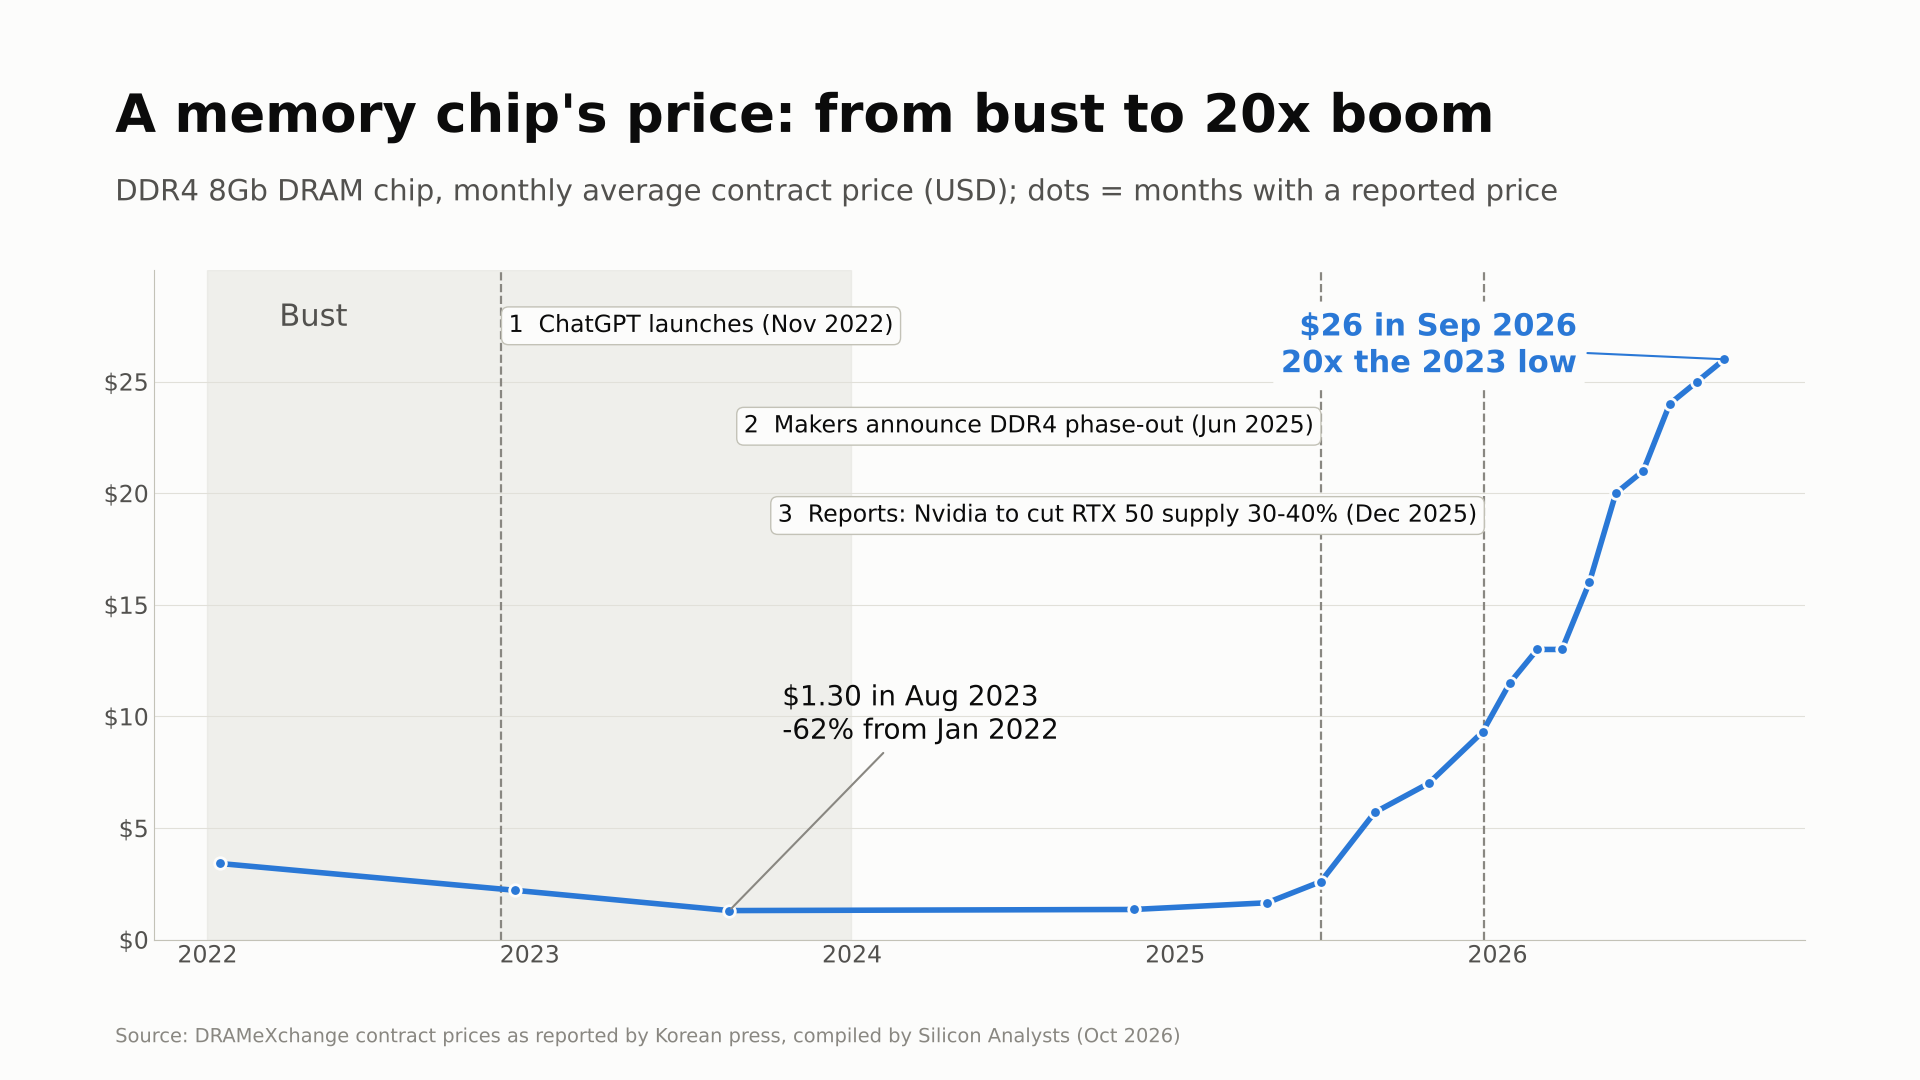
\includegraphics[width=0.72\linewidth]{figures/05_dram_price_cycle.png}
  \captionof{figure}{DDR4 8Gb contract price, Jan 2022 to Sep 2026, with three dated events.}
\end{center}

\section*{3. Technical challenges}

\begin{itemize}[leftmargin=1.2em]
  \item \textbf{Paywalled data:} we rebuilt the price series from monthly press reports and checked each value against its source.
  \item \textbf{Irregular sampling:} only 18 months have a price, so we plot dots on a true date axis to keep the gaps visible.
  \item \textbf{Mismatched sources:} capex datasets with different scopes stay in separate charts, with estimates marked.
  \item \textbf{A confounder:} DDR4 is being phased out, which inflates its rise; we flag this and cross-check with DDR5 prices.
  \item \textbf{Honest animation:} fixed scales and zero baselines in every clip, in one colourblind-safe palette.
\end{itemize}

\clearpage
\section*{4. Conclusion}

\begin{center}
  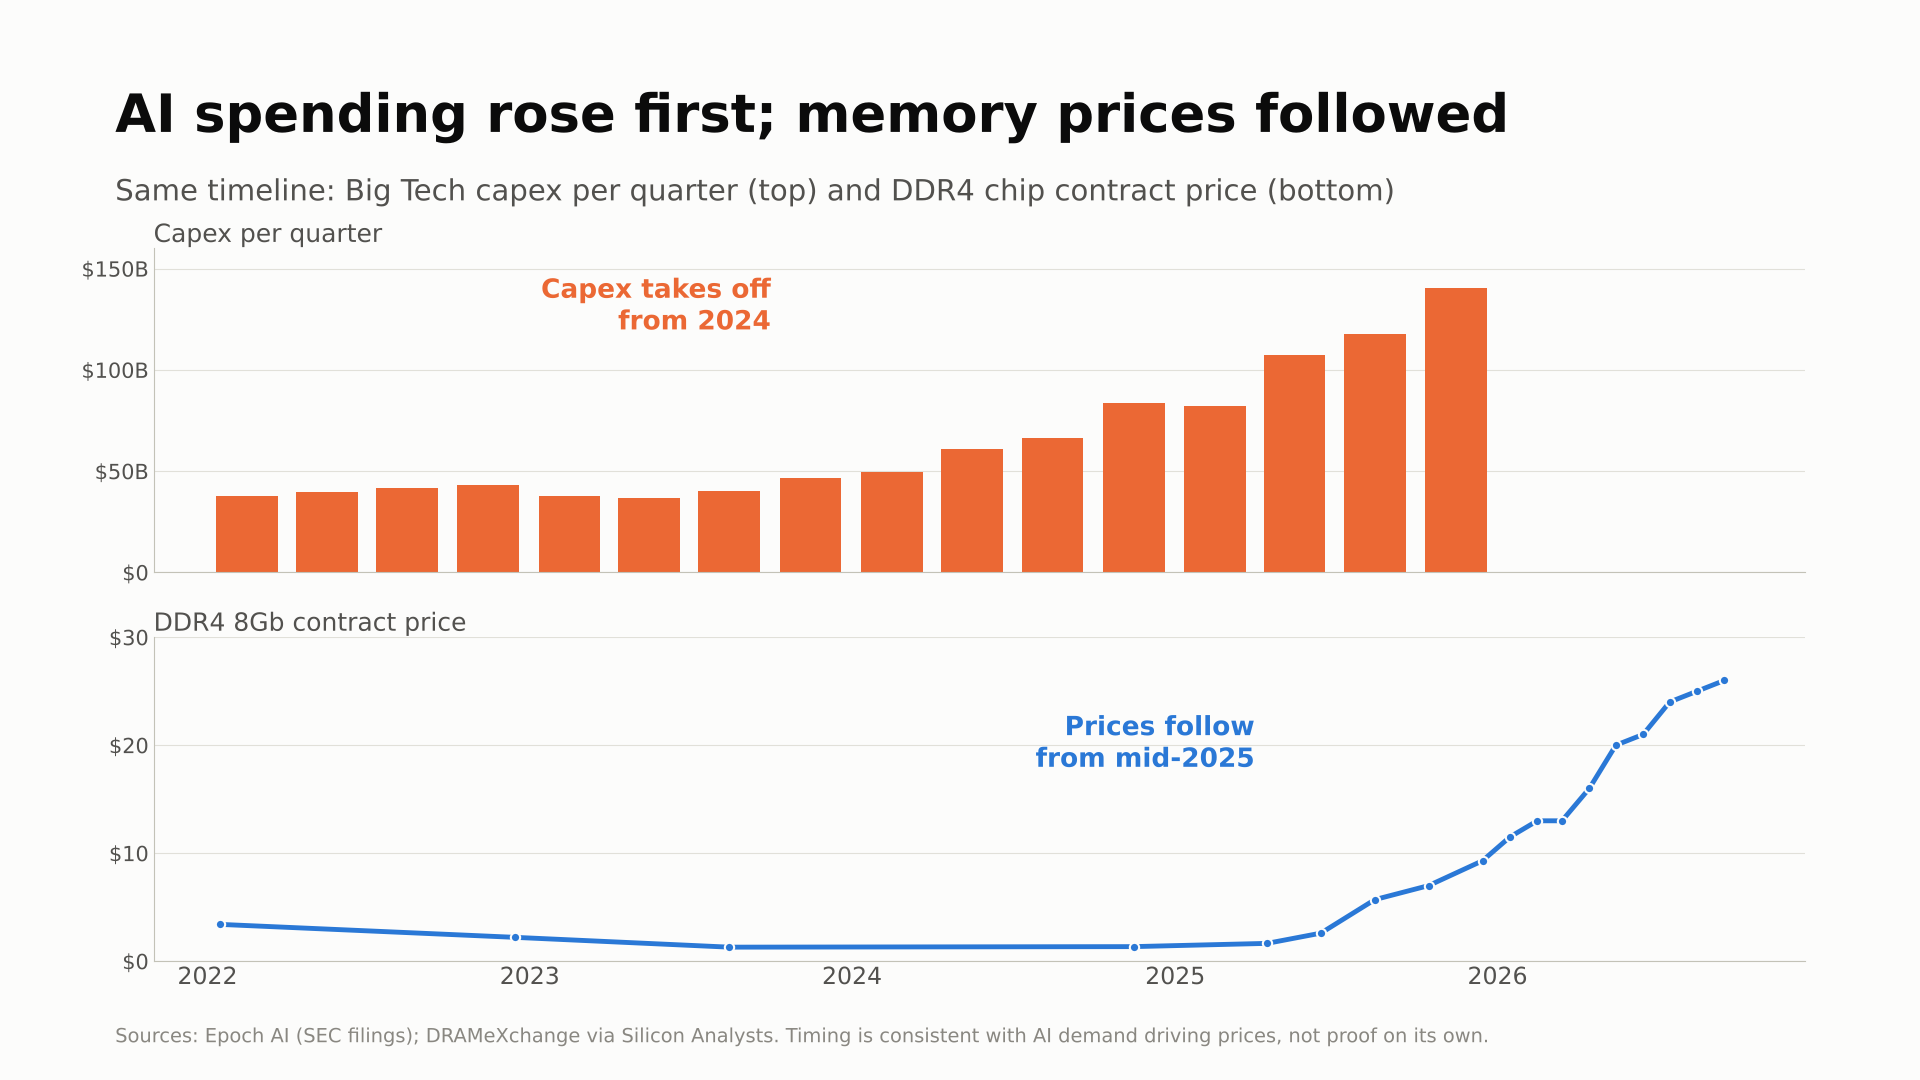
\includegraphics[width=0.72\linewidth]{figures/11_capex_vs_price.png}
  \captionof{figure}{Big Tech capex per quarter (top) and DDR4 contract price (bottom).}
\end{center}

The memory price surge is a side effect of the AI build-out: spending rose first, makers shifted capacity to AI, and prices followed. The squeeze reached consumers, including a reported 30--40\% cut in Nvidia RTX 50 supply. AI demand is real, but the build-out may run ahead of revenue. If spending slows, cyclical memory prices could fall as fast as they rose. Figure~2 shows the timing fits, though timing alone does not prove cause.

\section*{5. Contributions by each student}

\begin{tabularx}{\linewidth}{@{}p{2.6cm}p{2.5cm}X@{}}
\toprule
\textbf{Student} & \textbf{Matric ID} & \textbf{Contribution} \\
\midrule
Ayush Bhatt & G2610412E & Initial idea, initial draft, finding the datasets. \\
\addlinespace
Bu Dinglin & G2609929D & Idea brainstrom, visualisation modification, report finalisation and meeting organisation. \\
\bottomrule
\end{tabularx}

\vspace{0.6em}
{\footnotesize\color{muted} Sources: Silicon Analysts / DRAMeXchange; Epoch AI (SEC filings); SK hynix results releases; TrendForce; Gartner; Counterpoint Research; UBS via 24/7 Wall St.; Morgan Stanley via Benzinga; IoT Analytics. Full references in the report.}

\end{document}
